\chapter{Objetivos}
\label{chap:objetivos}

\noindent
%Para este capítulo, la normativa indica:
%
%«Concretar y exponer el problema a resolver describiendo el entorno de trabajo,
%la situación y detalladamente qué se pretende obtener. Limitaciones y
%condicionantes a considerar para la resolución del problema (lenguaje de
%construcción, equipo físico, equipo lógico de base y de apoyo, etc.). Si se
%considera necesario, esta sección puede titularse ``Objetivos e hipótesis de
%trabajo''. En este caso, se añadirán las hipótesis de trabajo que el alumno, con
%su TFG, pretende demostrar».

\drop{E}{n} este capítulo se expone el objetivo principal del \ac{TFG}, así como los objetivos parciales que se intentarán conseguir con la realización de este trabajo.

\section{Objetivo general}
El objetivo principal de este \ac{TFG} consiste en el desarrollo de un producto software que permita al usuario almacenar una posición geográfica (típicamente, el lugar de aparcamiento de uno o varios vehículos) y recuperar más tarde esta posición para mostrarla. El usuario podrá utilizar el producto bien desde un navegador web, accediendo y autenticándose en el servidor, bien a través del dispositivo móvil (ver figura \ref{fig:Preview_App}). En este último caso, se brinda la opción, una vez recuperada la posición, de mostrar una ruta guiada hasta el lugar de aparcamiento.

%Imagen App (Aproximacion)
\begin{figure}[h!btp]
\centering
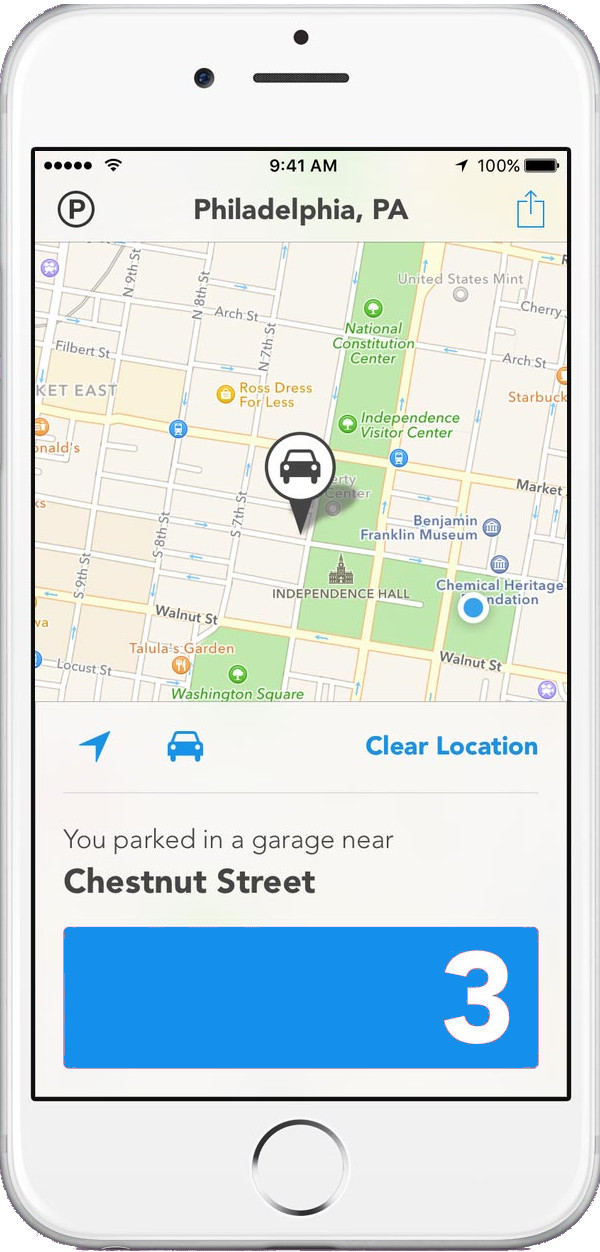
\includegraphics[height=60mm, fbox={\fboxrule} 4mm]{images/02-objetivos/01-telefono_parking.jpg}
\caption{Aproximación de la aplicación.}
\label{fig:Preview_App}
\end{figure}
%https://dotfirst.io/

\begin{tikzpicture}
	\node[shadowBox] {El objetivo del \ac{TFG} será la realización de una página web diseñada para almacenar y recuperar coordenadas geográficas y la modificación de las mismas por parte de varios usuarios.};
\end{tikzpicture}

En la figura \ref{fig:arquitectura} puede verse un diagrama de la arquitectura del sistema que se implementará en el presente \ac{TFG}.
\begin{figure}[h!btp]
\centering
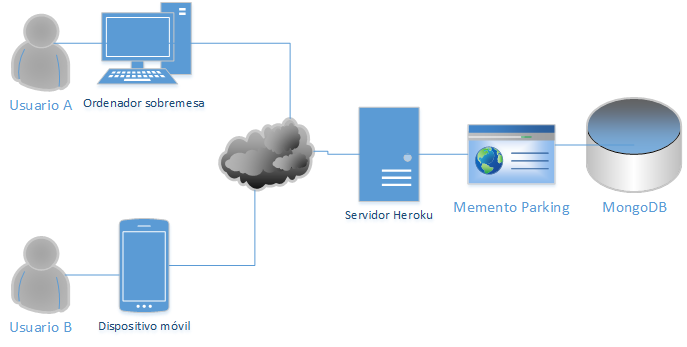
\includegraphics[scale=0.75, fbox={\fboxrule} 4mm]{images/02-objetivos/02-arquitectura.png}
\caption{Arquitectura de la aplicación}
\label{fig:arquitectura}
\end{figure}


\section{Objetivos específicos}

En la tabla \ref{tab:objetivos} se pueden observar los objetivos necesarios para la consecución del \ac{TFG}.

\begin{table}[hp]
  \centering 
  \rowcolors{1}{gray!25}{white}
  \begin{tabular}{p{0.2\linewidth}p{0.7\linewidth}}
    \multicolumn{1}{l}{\cellcolor{black!30}\textbf{Id Objetivo}} & 
 	\multicolumn{1}{c}{\cellcolor{black!30}\textbf{Descripción del objetivo}}\\
    \toprule
    Objetivo 1 & Realizar una página web para el acceso a la herramienta \\
	Objetivo 2 & Añadir gestión de usuarios a la página (registro y control de acceso) \\
	Objetivo 3 & Permitir el almacenamiento, edición y recuperación de datos a través de la página web \\
	Objetivo 4 & Mostrar los datos almacenados mediante la inclusión de un mapa \\
	Objetivo 5 & Facilitar a un usuario permitir a otros usuarios la edición de los datos almacenados \\
	Objetivo 6 & Añadir una opción para mostrar el recorrido desde el punto actual al punto almacenado \\
    \hline
  \end{tabular}
  \caption{Objetivos parciales del \ac{TFG}}
  \label{tab:objetivos}
\end{table}

\subsection{Objetivo 1}
\emph{Realizar una página web para el acceso a la herramienta.}\\
El comienzo del desarrollo será la implementación de una página web que sirva como marco y base para el resto de objetivos. Al término de este punto debe existir una página web accesible con todos los elementos típicos que un usuario espera encontrar, esto es, una página de inicio, contacto, acerca de, y una estructura reconocible y visualmente agradable. También se prestará atención a la accesibilidad desde dispositivos móviles comprobando que la visualización es correcta y no se pierde ni funcionalidad ni estética al cambiar el método de acceso. En la figura \ref{fig:prototipo_home} se puede observar un prototipo inicial de la página principal de la aplicación.

% IMAGEN: prototipo_Home
\begin{figure}[h!btp]
	\centering
	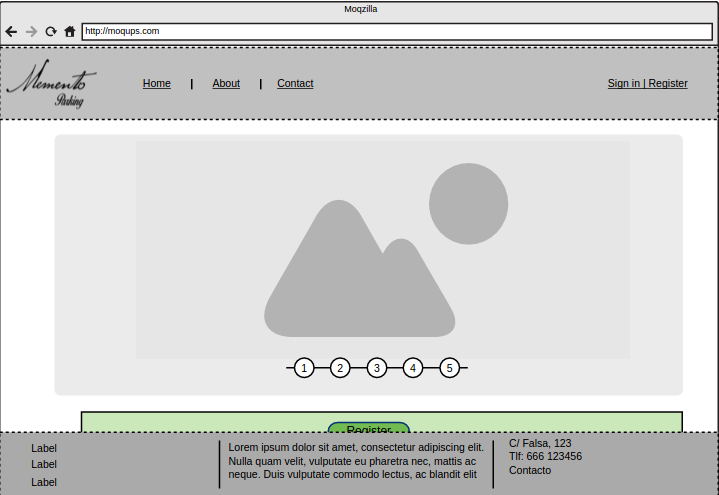
\includegraphics[scale=0.5, fbox={\fboxrule} 4mm]{images/02-objetivos/03-prototipo_home.png}
	\caption{Prototipo. Home}
	\label{fig:prototipo_home}
\end{figure}

\subsection{Objetivo 2}
\emph{Añadir gestión de usuarios a la página (registro y control de acceso).}\\
El segundo paso consistirá en realizar la gestión de usuarios permitiendo su registro y controlando el acceso de los mismos. Al terminar este punto la página web estará compuesta de contenido accesible a cualquier visitante y contenido accesible a aquellos usuarios autenticados en el sistema. Se prestará especial atención al almacenado seguro de las contraseñas mediante encriptación.

\subsection{Objetivo 3}
\emph{Permitir el almacenamiento, edición y recuperación de datos a través de la página web.}\\
El tercer objetivo consistirá en permitir al usuario almacenar las coordenadas introduciéndolas manualmente y mostrarlas por pantalla cuando así se requiera.

\subsection{Objetivo 4}
\emph{Mostrar los datos almacenados mediante la inclusión de mapa.}\\
El objetivo número cuatro refina la entrada de coordenadas permitiendo que el usuario no deba incluirlas a mano. Se mostrará un mapa por pantalla mediante el cual podrá seleccionarse una ubicación concreta para que el sistema recupere sus coordenadas geográficas y las almacene. La salida será similar, mostrándose las coordenadas mediante la inclusión de elementos reconocibles dentro del mapa (ver figura \ref{fig:prototipo_locations}).

% IMAGEN: prototipo_Locations
\begin{figure}[h!btp]
	\centering
	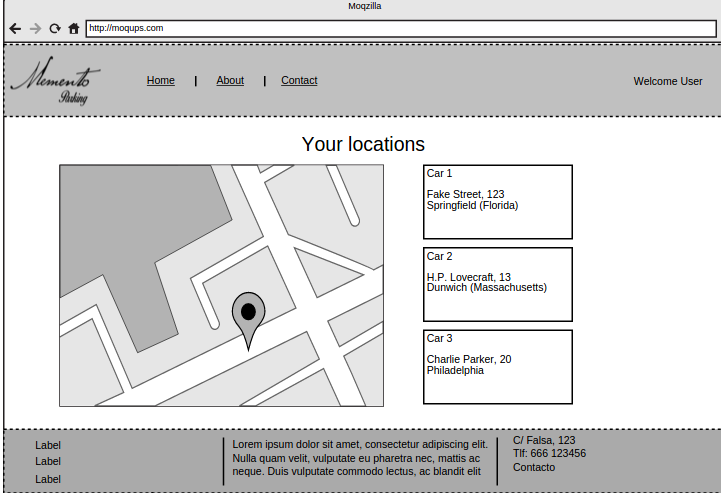
\includegraphics[scale=0.5, fbox={\fboxrule} 4mm]{images/02-objetivos/04-prototipo_locations.png}
	\caption{Prototipo. Localización}
	\label{fig:prototipo_locations}
\end{figure}


\subsection{Objetivo 5}
\emph{Facilitar a un usuario permitir que otros usuarios editen los datos almacenados.}\\
En este punto daremos un paso más en la gestión de usuarios permitiendo que interactúen entre ellos. El usuario propietario podrá dar permiso a ciertos usuarios, llamados \textit{usuarios conocidos}, para acceder a sus datos almacenados y poder modificarlos.


\subsection{Objetivo 6}
\emph{Añadir una opción para mostrar el recorrido desde el punto actual al punto almacenado.}\\
El objetivo final será añadir funcionalidades auxiliares, como es mostrar una ruta desde la localización del usuario hasta la posición almacenada.

\section{Objetivos académicos}
La consecución del \ac{TFG} lleva una serie de objetivos académicos aparejados, entre los que cabe destacar el aprendizaje y asentamiento de las siguientes tecnologías:

\begin{itemize}[label={$\bullet$},labelindent=\parindent,leftmargin=2cm]
	\item Ruby on Rails
	\item MongoDB
	\item AngularJS
	\item Bootstrap
	\item Android
\end{itemize}

% Local Variables:
%  coding: utf-8
%  mode: latex
%  mode: flyspell
%  ispell-local-dictionary: "castellano8"
% End:
